\section{Results}

\subsection{Median over the designs}

We first compared the pass rates of the 32 designs under independent deposition errors. Each point is based on 200 simulated mirrors, and the rescue re-designed the top four layers, with perfect measurement or with measurement errors of 1\% and 2\%. Figure~\ref{fig:typical} shows the median pass rate over the 32 designs as the deposition error grows; the shaded bands show the middle half of the designs.

Without rescue, the median pass rate was 99\% at $\sigma = 1\%$, 76\% at 2\%, and 49\% at 3\%. With rescue and perfect measurement, these rose to 100\%, 92\% and 67\%.

With 2\% measurement error the picture changed. The median pass rate was only 93\% even at $\sigma = 0.25\%$, where every mirror of every design passed without rescue.

\begin{figure}[t]
\centering
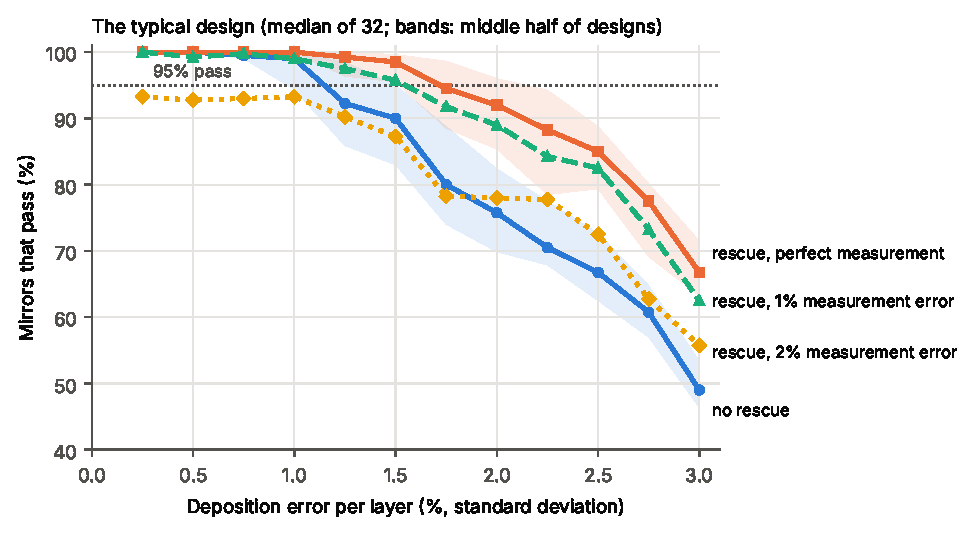
\includegraphics[width=0.75\linewidth]{fig1_typical_design}
\caption{Median pass rate of the 32 designs against deposition error $\sigma$ (independent errors, 200 mirrors per point, top four layers rescued, every mirror rescued). Bands: middle half of the designs, without rescue and with rescue at perfect measurement.}
\label{fig:typical}
\end{figure}

\subsection{How much the rescue raises the tolerable error}
\label{sec:q1}

For each design we found the tolerable error, the deposition error at which the pass rate falls to 95\%, with and without rescue (Fig.~\ref{fig:every}, left).

Without rescue, the median tolerable error was 1.14\%, with the middle half of the designs between 0.96\% and 1.48\%. With rescue and perfect measurement, the median rose to 1.71\% (middle half 1.52--2.19\%). The rescue raised the tolerable error in 30 of the 32 designs, and in 27 of them the uncertainty ranges did not overlap. A sign test gives $p = 2\times10^{-7}$ for 30 increases and 2 decreases. The median per-design gain was 0.59~pp (95\% interval 0.49--0.67~pp; Wilcoxon $p = 10^{-8}$). Expressed as a ratio, the median gain was a factor of 1.43 (95\% interval 1.36--1.56), and it varied between designs from 0.68 to 2.04.

Two designs did worse after rescue. For S1 the tolerable error fell from 0.96\% to 0.66\%, and the uncertainty ranges did not overlap. For E1 it fell from 0.90\% to 0.86\%, with overlapping ranges.

The result does not depend on the three exploratory designs or on the 95\% threshold. Without E1--E3, the median rose from 1.13\% to 1.72\%, with 28 designs up and 1 down. With a 90\% threshold, it rose from 1.43\% to 2.10\%, with 30 up and 2 down.

Designs that were sturdier without rescue did not clearly gain more from it: the rank correlation was $\rho = 0.30$ ($p = 0.09$; corrected $p = 0.6$).

At a single deposition error of 2\%, the median pass rate rose from 76\% without rescue to 92\% with rescue and perfect measurement. All 32 designs had a higher pass rate after rescue, and the number of designs reaching 95\% went from 1 to 13. A second, independent set of 200 mirrors per design gave the same picture: again all 32 designs improved, with a median gain of 12.5 percentage points against 12.2 for the first set.

E3 was also scanned separately with 400 mirrors per point. With 200 mirrors its tolerable error rose from 1.79\% to 2.54\%, and with 400 mirrors from 1.69\% to 2.65\%; the uncertainty ranges overlap. E3 is the third sturdiest of the 32 designs, but its gain ratio with 200 mirrors (1.42) is close to the median.

\begin{figure}[t]
\centering
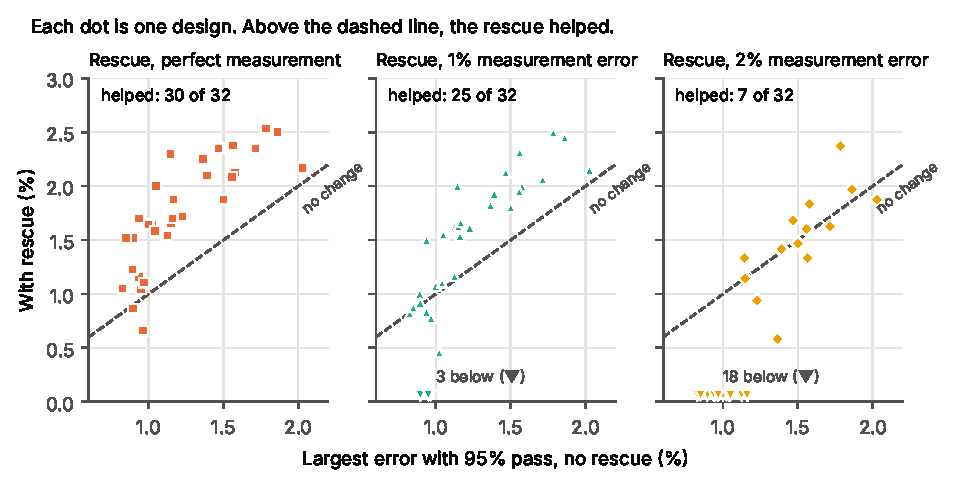
\includegraphics[width=\linewidth]{fig2_every_design}
\caption{Tolerable error of every design with rescue (vertical) against without rescue (horizontal), at three measurement-error levels. Each point is one design; above the dashed line the rescue helped. Triangles at the bottom: designs whose pass rate was below 95\% already at $\sigma = 0.25\%$.}
\label{fig:every}
\end{figure}

\subsection{Effect of measurement error}
\label{sec:measres}

Table~\ref{tab:meas} and Fig.~\ref{fig:every} (middle and right) show how measurement error changes the result. With 1\% measurement error, the rescue still raised the tolerable error in 25 designs and lowered it in 7; the median was 1.58\% (median per-design gain 0.36~pp, 95\% interval 0.07--0.48~pp). With 2\% measurement error, it lowered the tolerable error in 25 designs and raised it in 7. For 18 of the 32 designs, the pass rate with rescue was below 95\% even at the smallest deposition error tested, 0.25\%, so the median tolerable error was below 0.25\%.

At 2\% measurement error the two ways of measuring the effect disagree. The tolerable error is set by small deposition errors, where almost every mirror passes without rescue and the rescue can only do harm. At $\sigma = 2\%$, where there is more to fix, the rescue was roughly neutral: 15 designs had a higher pass rate and 13 a lower one ($p = 0.85$), and mirror by mirror it saved 547 mirrors and broke 609. With a 90\% threshold the tolerable error fell in 19 designs and rose in 13 ($p = 0.4$). With perfect measurement, by contrast, the rescue saved 848 mirrors and broke 38, and was significantly better for 28 designs after correction for multiple tests and significantly worse for none. With 1\% measurement error it saved 759 and broke 190 (25 designs better, 1 worse).

\begin{table}[t]
\centering
\caption{Effect of measurement error on the rescue (independent deposition errors, 32 designs, every mirror rescued). Tolerable error: median and middle half of the designs. ``Clear'': non-overlapping 95\% ranges. Mirrors saved and broken, and designs significantly better or worse after Holm correction, are from the paired comparison at $\sigma = 2\%$. Without rescue, the median tolerable error is 1.14\% (0.96--1.48\%).}
\label{tab:meas}
\footnotesize\setlength{\tabcolsep}{4pt}
\begin{tabular}{lccccc}
\toprule
Measurement & Tolerable error & Raised (clear) / & Sign test & Mirrors saved / & Designs better / \\
error & median (middle half) & lowered (clear) & $p$ & broken & worse \\
\midrule
0\% & 1.71\% (1.52--2.19\%) & 30 (27) / 2 (1) & $2\times10^{-7}$ & 848 / 38 & 28 / 0 \\
1\% & 1.58\% (0.91--1.96\%) & 25 (14) / 7 (3) & 0.002 & 759 / 190 & 25 / 1 \\
2\% & $<0.25\%$ ($<0.25$--1.43\%) & 7 (1) / 25 (18) & 0.002 & 547 / 609 & 1 / 2 \\
\bottomrule
\end{tabular}
\end{table}

To find where the rescue stops helping, we added measurement errors of 0.5\% and 1.5\% (Table~\ref{tab:thresh}). The answer depends on the deposition error. At $\sigma = 1\%$, the rescue helped with measurement errors up to 0.5\%, was neutral at 1\%, and did harm from 1.5\%. At $\sigma = 2\%$, it helped up to 1.5\% and was neutral at 2\%. At $\sigma = 0.25\%$ and 0.5\%, where nearly every mirror passes anyway, any measurement error of 1\% or more did harm. In every case the rescue helped clearly only when the measurement error was smaller than the deposition error. At the points where we repeated the runs with a second set of mirrors, the counts agreed within a few designs (Sec.~\ref{sec:checksres}).

\begin{table}[t]
\centering
\caption{Designs whose pass rate rose / fell with rescue, compared with no rescue on the same 200 mirrors (independent errors, 32 designs, every mirror rescued). Bold: the rescue helped (sign test $p < 0.05$); italic: it did harm.}
\label{tab:thresh}
\footnotesize
\begin{tabular}{lccccc}
\toprule
 & \multicolumn{5}{c}{Measurement error} \\
Deposition error $\sigma$ & 0\% & 0.5\% & 1\% & 1.5\% & 2\% \\
\midrule
0.25\% & 0 / 0 & 0 / 2 & \emph{0 / 13} & \emph{0 / 20} & \emph{0 / 27} \\
0.5\% & 0 / 1 & 0 / 4 & \emph{0 / 18} & \emph{0 / 23} & \emph{0 / 28} \\
1\% & \textbf{18 / 2} & \textbf{16 / 2} & 12 / 8 & \emph{1 / 22} & \emph{0 / 30} \\
2\% & \textbf{32 / 0} & \textbf{31 / 1} & \textbf{28 / 4} & \textbf{22 / 6} & 15 / 13 \\
\bottomrule
\end{tabular}
\end{table}

Part of the harm comes from rescuing every mirror, including mirrors that would have passed. With the gated rule, which rescues only mirrors whose measurements predict a failure, the median tolerable error at 2\% measurement error was 0.93\% instead of below 0.25\%, and 9 designs were ``below'' instead of 18. It was still lower than without rescue (1.14\%): it fell in 21 designs and rose in 10 (Wilcoxon $p = 0.001$). With measurements this poor, the gate itself makes mistakes. It flags good mirrors as failing and rescues them into failure; at $\sigma = 0.25\%$ the median pass rate with the gated rule was 97\%, and one design fell to 72\%. With better measurement, gating gave up part of the gain. Its median tolerable error was 1.59\% with perfect measurement (always rescuing: 1.71\%) and 1.29\% with 1\% measurement error (always rescuing: 1.58\%), because a mirror predicted to pass can still fail once its top layers are deposited with their own errors.

Sturdier designs lost less when measurement got worse. The rank correlation between a design's tolerable error without rescue and its loss in tolerable error from 0\% to 2\% measurement error was $\rho = -0.52$ ($p = 0.002$; corrected $p = 0.02$). This value depends on how ``below'' is entered: with 0.25\% instead of 0 it is $\rho = -0.42$ ($p = 0.02$). At the single deposition error of 2\%, the same correlation, using pass rates, was $\rho = -0.87$ (corrected $p = 10^{-9}$).

\subsection{Quieter and noisier designs}

Without rescue, designs with lower thermal noise tolerated smaller deposition errors: the rank correlation between the noise proxy and the tolerable error was $\rho = 0.67$ ($p = 3\times10^{-5}$; corrected $p = 0.0004$). Much of this correlation comes from the gap between the two noise groups described in Methods. Within the quiet group the correlation was strong ($\rho = 0.72$); within the noisy group it was weak and not significant ($\rho = 0.26$, $p = 0.37$).

Without rescue, the median tolerable errors of the quiet group (18 designs) and the noisy group (14 designs) were 1.00\% and 1.31\%. With rescue and perfect measurement they rose to 1.56\% and 2.09\%, raising the tolerable error in 17 of 18 quiet designs and 13 of 14 noisy ones. The rescued quiet designs therefore tolerated more error than the noisy designs without rescue. With 1\% measurement error, the quiet group fell to 1.05\%, while the noisy group kept 1.86\%. With 2\% measurement error, 14 of the 18 quiet designs were ``below'', against 4 of the 14 noisy designs; the noisy group's median was 1.33\%.

\subsection{Shared deposition errors}

So far each layer had its own error. With a shared error, all 40 layers are off by the same fraction. Table~\ref{tab:shared} and Fig.~\ref{fig:shared} compare the two cases.

At 1\% shared error, the median pass rate without rescue was 66\%. With rescue it rose to 76\% with perfect measurement, 74\% with 1\% measurement error and 69\% with 2\%. At 2\% shared error, the median was 40.5\% without rescue and 48\%, 46\% and 42\% with rescue. With perfect measurement, the rescue raised the pass rate of 31 designs at 1\% shared error and of 29 at 2\%. No design reached a 95\% pass rate: the best after rescue was 91.5\% at 1\% and 56\% at 2\%.

The gain at 1\% shared error is small but consistent. The sign test gives $p = 2\times10^{-8}$. Mirror by mirror, the rescue saved 700 mirrors and broke 29; it was significantly better for 27 designs after correction and significantly worse for none. At 2\% shared error, sturdier designs gained less from the rescue with perfect measurement ($\rho = -0.66$, corrected $p = 0.0005$).

Re-designing more layers helped, but not enough. At 1\% shared error with perfect measurement, the median pass rate was 72.5\% with $k = 2$, 75.5\% with $k = 4$, 79\% with $k = 6$, 83\% with $k = 8$ and 88\% with $k = 12$. Twelve layers did better than four for 31 of the 32 designs, but only 2 designs reached 95\%. A global optimizer did not change this either (Sec.~\ref{sec:checksres}). A shared error scales every layer by the same factor, which shifts the whole spectrum of the coating in wavelength. The top layers can change the phase of the light reflected from the stack beneath them, but they cannot shift that stack's spectrum back, so a few layers can only partly undo the error.

\begin{table}[t]
\centering
\caption{Pass rates under independent and shared deposition errors (32 designs, 200 mirrors each, $k = 4$). Medians over designs; ``raised'' counts designs whose pass rate rose with rescue at perfect measurement.}
\label{tab:shared}
\footnotesize\setlength{\tabcolsep}{4pt}
\begin{tabular}{lccccc}
\toprule
 & No rescue & Rescue, meas.\ 0 / 1 / 2\% & Raised & Best after rescue & Reached 95\% \\
\midrule
Independent, 2\% & 76\% & 92 / 89 / 78\% & 32 & 99.5\% & 13 \\
Shared, 1\% & 66\% & 76 / 74 / 69\% & 31 & 91.5\% & 0 \\
Shared, 2\% & 40.5\% & 48 / 46 / 42\% & 29 & 56\% & 0 \\
\bottomrule
\end{tabular}
\end{table}

\begin{figure}[t]
\centering
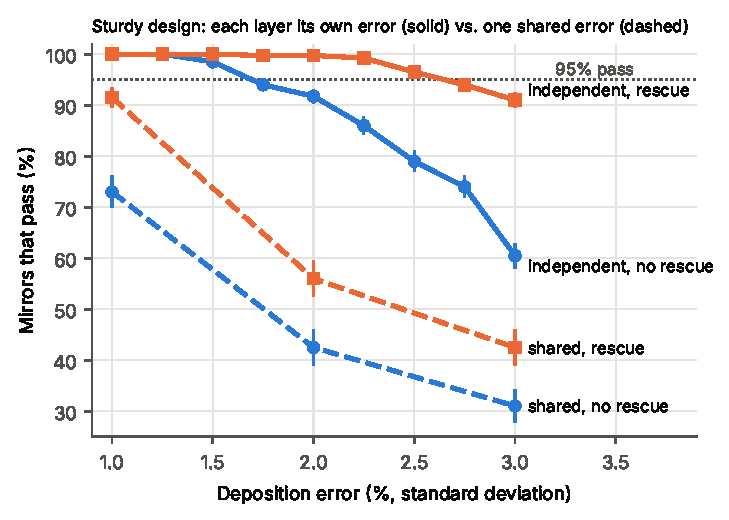
\includegraphics[width=0.9\linewidth]{fig3_shared_error}
\caption{Pass rate of every design without and with rescue ($k = 4$, perfect measurement). Grey lines join the same design; the black line joins the medians. Dotted line: 95\% pass.}
\label{fig:shared}
\end{figure}

\subsection{Number of rescued layers}
\label{sec:kres}

All results above use $k = 4$. Under independent errors of 2\% with perfect measurement, re-designing more layers helped up to about six to eight (Table~\ref{tab:k}). The median pass rate was 92\% with $k = 4$ and 96\% with $k = 8$, and the number of designs reaching 95\% rose from 13 to 20. With $k = 12$ the median fell back to 93.5\%, although the worst design improved. The best $k$ was 6 for 13 designs, 8 for 7 and 12 for 10. The choice $k = 4$ therefore understates what the rescue can do under independent errors.

\begin{table}[t]
\centering
\caption{Pass rate against the number of rescued layers $k$ (32 designs, 200 mirrors each, perfect measurement). Medians over designs.}
\label{tab:k}
\footnotesize
\begin{tabular}{lccccc}
\toprule
$k$ & 2 & 4 & 6 & 8 & 12 \\
\midrule
Independent 2\%: median pass rate & 83\% & 92\% & 95.5\% & 96\% & 93.5\% \\
\quad designs reaching 95\% & 4 & 13 & 20 & 20 & 11 \\
Shared 1\%: median pass rate & 72.5\% & 75.5\% & 79\% & 83\% & 88\% \\
\quad designs reaching 95\% & 0 & 0 & 0 & 0 & 2 \\
\bottomrule
\end{tabular}
\end{table}

\subsection{Why mirrors fail}

We classified the failed mirrors of one design, E3 (Fig.~\ref{fig:failures}). This is a single-design example, not a population result, and it uses its own set of mirrors.

Without rescue, most failures came from 532~nm transmission above its 4\% limit. The rescue removed most of these, and the remaining failures were mainly from 1064~nm transmission above 6~ppm. For example, at 3\% independent error, 40 mirrors failed only the 532~nm limit, 17 only the 1064~nm limit, and 18 both; after rescue these numbers were 5, 16 and 0. At 2\% shared error, the largest group failed both limits at once, and the rescue removed few of these (63 to 55). Failures almost always came from too much transmission, almost never from too little.

\begin{figure}[t]
\centering
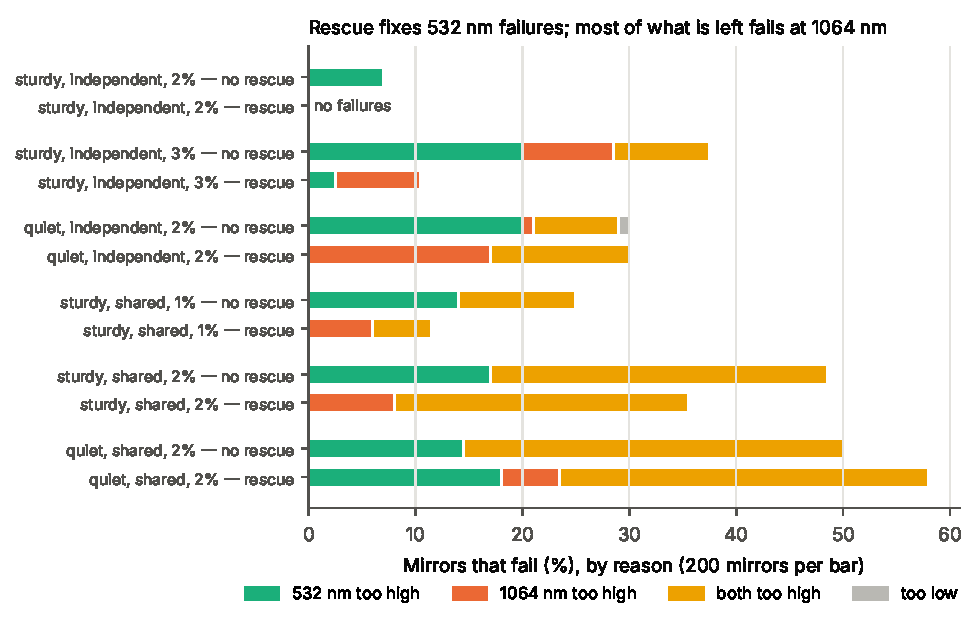
\includegraphics[width=0.75\linewidth]{fig4_failures}
\caption{Failed mirrors of design E3 by the limit they missed, without and with rescue ($k = 4$, perfect measurement), 200 mirrors per bar.}
\label{fig:failures}
\end{figure}

\subsection{Thermal noise}
\label{sec:noiseres}

We computed the full Brownian noise of every mirror at $\sigma = 2\%$ (independent errors), with and without rescue, for all 32 designs. With perfect measurement, the rescue changed the noise at 100~Hz by a median of $-0.02\%$. Ninety percent of mirrors changed by between $-0.63\%$ and $+0.30\%$, and the largest increase for any mirror was 1.09\%. The median of single designs ranged from $-0.24\%$ to $+0.12\%$. With 1\% and 2\% measurement error the medians were $-0.01\%$ and $-0.003\%$, and the largest increases 1.06\% and 1.16\%. Using a substrate Young's modulus of 72.7~GPa instead of 60~GPa changed the median to $-0.01\%$. The noise proxy gave a median of $-0.035\%$ with perfect measurement, twice the full calculation, but both are far below 1\%.

\subsection{Method checks}
\label{sec:checksres}

\emph{Optimizer.} In the first check, on E1 and E3, the slow differential-evolution rescue passed 22 mirrors that L-BFGS-B failed, and L-BFGS-B passed 5 that the slow one failed, out of 1600 (exact McNemar $p = 0.0015$). So the fast optimizer does miss some rescues. Nineteen of the 22 were E1 mirrors under shared errors; for E3 there were 4 disagreements in 800 mirrors. On all 32 designs at 1\% shared error, the two optimizers gave median pass rates of 75.0\% (differential evolution) and 75.5\% (L-BFGS-B). Differential evolution did better for 7 designs, worse for 2, and the same for 23 ($p = 0.18$), and its largest gain on any design was 3.5 percentage points. The fast optimizer's misses are real but too small to explain why shared errors cannot be fixed.

\emph{Second set of mirrors.} We repeated the runs at independent $\sigma = 0.25\%$ and 2\% and shared $\sigma = 1\%$ and 2\%, at all three measurement errors, with a new set of 200 mirrors per design. Every comparison went the same way as with the first set. For example, at independent $\sigma = 2\%$ with 1\% measurement error the rescue raised the pass rate of 29 designs and lowered it for 3 (first set: 28 and 4), and at 2\% measurement error it was neutral again (17 and 14; first set: 15 and 13). The designs that gained most were the same in both sets (rank correlation of the gains between the two sets, 0.64--0.98).

\emph{Size of the Advanced LIGO error.} Scaling all layer thicknesses by a common factor showed how large a systematic error must be to raise the 532~nm transmission tenfold, as happened in the Advanced LIGO end mirrors~\cite{aLIGO2015}: $-2.25\%$ for E3 and $-1.00\%$ for E1. In our model this scaling also pushed the 1064~nm transmission out of its window, which did not happen in the real mirrors. The 1064~nm transmission stayed in range only when one material was scaled; scaling only the silica layers gave 5.21~ppm (E3, $+6.00\%$) and 5.85~ppm (E1, $-1.50\%$). The real coating design differed from ours, so this check shows that errors of a few percent are enough, not that it reproduces the real event.
